\lab{Pandas IV: Time Series}{Pandas IV: Time Series}
\objective{Many real world data sets---stock market measurements, ocean tide levels, website traffic, seismograph data, audio signals, fluid simulations, quarterly dividends, and so on---are time series, meaning they come with time-based labels.
There is no universal format for such labels, and indexing by time is often difficult with raw data.
Fortunately, pandas has tools for cleaning and analyzing time series.
In this lab we use pandas to clean and manipulate time-stamped data and introduce some basic tools for time series analysis.}

% Time series data is any form of data that comes attached to a timestamp (i.e. Sept 28, 2016 20:32:24) or a period of time (i.e. Q3 2012). Some examples of time series data include:

\section*{Working with Dates and Times} % =====================================

The \li{datetime} module in the standard library provides a few tools for representing and operating on dates and times.
The \li{datetime.datetime} object represents a \emph{time stamp}: a specific time of day on a certain day.
Its constructor accepts a four-digit year, a month (starting at 1 for January), a day, and, optionally, an hour, minute, second, and microsecond.
Each of these arguments must be an integer, with the hour ranging from $0$ to $23$ (military time).

\begin{lstlisting}
>>> from datetime import datetime

# Represent November 18th, 1991, at 2:01 PM.
>>> bday = datetime(1991, 11, 18, 14, 1)
>>> print(bday)
1991-11-18 14:01:00

# Find the number of days between 11/18/1991 and 11/9/2017.
>>> dt = datetime(2017, 11, 9) - bday
>>> dt.days
9487
\end{lstlisting}

The \li{datetime.datetime} object has a parser method, \li{strptime()}, that converts a string into a new \li{datetime.datetime} object.
The parser is flexible because the user must specify the format that the dates are in.
For example, if the dates are in the format \li{"Month/Day//Year::Hour"}, specify \li{<<format>>="\%m/\%d//\%Y::\%H"} to parse the string appropriately.
See Table \ref{table:date_formats} for formatting options.

\begin{table}[H]
\begin{center}
    \begin{tabular}{c|l}
        Pattern & Description \\ \hline
        \li{\%Y} & 4-digit year \\
        \li{\%y} & 2-digit year \\
        \li{\%m} & 1- or 2-digit month \\
        \li{\%d} & 1- or 2-digit day \\
        \li{\%H} & Hour (24-hour) \\
        \li{\%I} & Hour (12-hour) \\
        \li{\%M} & 2-digit minute \\
        \li{\%S} & 2-digit second \\
    \end{tabular}
\end{center}
\caption{Formats recognized by \li{datetime.strptime()}}
\label{table:date_formats}
\end{table}

\begin{lstlisting}
>>> print(datetime.strptime("1991-11-18 / 14:01", "%Y-%m-%d / %H:%M"),
...       datetime.strptime("1/22/1996", "%m/%d/%Y"),
...       datetime.strptime("19-8, 1998", "%d-%m, %Y"), sep='\n')
1991-11-18 14:01:00                 # The date formats are now standardized.
1996-01-22 00:00:00                 # If no hour/minute/seconds data is given,
1998-08-19 00:00:00                 #  the default is midnight.
\end{lstlisting}

\subsection*{Converting Dates to an Index} % ----------------------------------

The \li{TimeStamp} class is the pandas equivalent to a \li{datetime.datetime} object.
An pandas index for composed of \li{TimeStamp} objects is a \li{DatetimeIndex}, and a \li{Series} or \li{DataFrame} with such an index is called a \emph{time series}.
The function \li{pd.to_datetime()} converts a collection of dates in a parsable format to a \li{DatetimeIndex}.
The format of the dates is inferred if possible, but it can be specified explicitly with the same syntax as \li{datetime.strptime()}.

\begin{lstlisting}
>>> import pandas as pd

# Convert some dates (as strings) into a DatetimeIndex.
>>> dates = ["2010-1-1", "2010-2-1", "2012-1-1", "2012-1-2"]
>>> pd.to_datetime(dates)
<<DatetimeIndex(['2010-01-01', '2010-02-01', '2012-01-01', '2012-01-02'],
                dtype='datetime64[ns]', freq=None)>>

# Create a time series, specifying the format for the dates.
>>> dates = ["1/1, 2010", "1/2, 2010", "1/1, 2012", "1/2, 2012"]
>>> date_index = pd.to_datetime(dates, format="%m/%d, %Y")
>>> pd.Series([x**2 for x in range(4)], index=date_index)
<<2010-01-01    0
2010-01-02    1
2012-01-01    4
2012-01-02    9
dtype: int64>>
\end{lstlisting}

\begin{comment}
\begin{warn} % Deprecated TimeSeries object.
Prior to version 0.17.0 of \li{pandas}, there was a dedicated \li{TimeSeries} data structure.
This has since been deprecated in favor of the more general \li{Series} and \li{DataFrame} data structures.
Any materials referencing the \li{TimeSeries} can be corrected by replacing the \li{TimeSeries} with a \li{Series} or \li{DataFrame} with a \li{DatetimeIndex} as the index.
\end{warn}
\end{comment}

\begin{problem} % Load, clean, and plot Dow Jones IA data.
The file \texttt{DJIA.csv} contains daily closing values of the Dow Jones Industrial Average from 2006--2016.
Read the data into a \li{Series} or \li{DataFrame} with a \li{DatetimeIndex} as the index.
Drop rows with missing values, cast the \li{"VALUES"} column to floats, then plot the data.
\\(Hint: Use \li{lw=.5} to make the line thin enough for the data.)
\label{prob:timeseries-dowjones}
\end{problem}

\subsection*{Generating Time-based Indices} % ---------------------------------

Some time series datasets come without explicit labels, but still have instructions for deriving timestamps.
For example, a list of bank account balances might have records from the beginning of every month, or heart rate readings could be recorded by an app every 10 minutes.
Use \li{pd.date\_range()} to generate a \li{DatetimeIndex} where the timestamps are equally spaced.
The function is analogous to \li{np.arange()} and has the following parameters.
\begin{table}[H]
\begin{center}
    \begin{tabular}{r|l}
        Parameter & Description \\ \hline
        \li{start} & Starting date \\
        \li{end} & End date \\
        \li{periods} & Number of dates to include \\
        \li{freq} & Amount of time between consecutive dates \\
        \li{normalize} & Whether or not to trim the time to midnight \\
    \end{tabular}
\end{center}
\caption{Parameters for \li{pd.date_range()}.}
\label{table:date_params}
\end{table}

Exactly two of the parameters \li{start}, \li{end}, and \li{periods} must be specified to generate a range of dates.
The \li{freq} parameter accepts a variety of string representations, referred to as \emph{offset aliases}.
See Table \ref{table:range_freqs} for a sampling of some of the options.
For a complete list of the options, see \url{http://pandas.pydata.org/pandas-docs/stable/timeseries.html#offset-aliases}.

\begin{table}[H]
\begin{center}
    \begin{tabular}{r|l}
        Parameter & Description \\ \hline
        \li{"D"} & calendar daily (default) \\
        \li{"B"} & business daily \\
        \li{"H"} & hourly \\
        \li{"T"} & minutely \\
        \li{"S"} & secondly \\
        \li{"MS"} & first day of the month \\
        \li{"BMS"} & first weekday of the month \\
        \li{"W-MON"} & every Monday \\
        \li{"WOM-3FRI"} & every 3rd Friday of the month \\
    \end{tabular}
\end{center}
\caption{Options for the \li{freq} parameter to \li{pd.date_range()}.}
\label{table:range_freqs}
\end{table}

\begin{lstlisting}
# 5 consecutive days staring with September 28, 2016.
>>> pd.date_range(start='9/28/2016 16:00', periods=5)
<<DatetimeIndex(['2016-09-28 16:00:00', '2016-09-29 16:00:00',
               '2016-09-30 16:00:00', '2016-10-01 16:00:00',
               '2016-10-02 16:00:00'],
              dtype='datetime64[ns]', freq='D')>>

# The first weekday of every other month in 2016.
>>> pd.date_range(start='1/1/2016', end='1/1/2017', freq="2BMS" )
<<DatetimeIndex(['2016-01-01', '2016-03-01', '2016-05-02', '2016-07-01',
               '2016-09-01', '2016-11-01'],
              dtype='datetime64[ns]', freq='2BMS')>>


# 10 minute intervals between 4:00 PM and 4:30 PM on September 9, 2016.
>>> pd.date_range(start='9/28/2016 16:00',
            end='9/28/2016 16:30', freq="10T")
<<DatetimeIndex(['2016-09-28 16:00:00', '2016-09-28 16:10:00',
               '2016-09-28 16:20:00', '2016-09-28 16:30:00'],
              dtype='datetime64[ns]', freq='10T')>>
\end{lstlisting}

The \li{freq} parameter also supports more flexible string representations.

\begin{lstlisting}
>>> pd.date_range(start='9/28/2016 16:30', periods=5, freq="2h30min")
<<DatetimeIndex(['2016-09-28 16:30:00', '2016-09-28 19:00:00',
               '2016-09-28 21:30:00', '2016-09-29 00:00:00',
               '2016-09-29 02:30:00'],
              dtype='datetime64[ns]', freq='150T')>>
\end{lstlisting}

\begin{problem} % Use pd.date_range() for something.
The file \texttt{paychecks.csv} contains values of an hourly employee's last 93 paychecks.
He started working March 13, 2008.
This company hands out paychecks on the first and third Fridays of the month.

Read in the data, using \li{pd.date\_range()} to generate the \li{DatetimeIndex}.
Plot the data.
\\(Hint: use the \li{union()} method of \li{DatetimeIndex} class.)
\end{problem}

\section*{Periods} % ==========================================================

The pandas \li{Timestamp} object represents a precise moment in time on a given day.
Some data, however, is recorded over a time interval, and it wouldn't make sense to place an exact timestamp on any of the measurements.
For example, a record of the number of steps walked in a day, box office earnings per week, quarterly earnings, and so on.
This kind of data is better represented with the pandas \li{Period} object and the corresponding \li{PeriodIndex}.

The constructor of the \li{Period} accepts a \li{value} and a \li{freq}.
The \li{value} parameter indicates the label for a given \li{Period}.
This label is tied to the \textbf{end} of the defined \li{Period}.
The \li{freq} indicates the length of the \li{Period} and also (in some cases) indicates the offset of the \li{Period}.
The \li{freq} parameter accepts the majority, but not all, of frequencies listed in Table \ref{table:range_freqs}.

\begin{lstlisting}
# The default value for 'freq' is "M" for months.
>>> p1 = pd.Period("2016-10")
>>> p1.start_time                   # The start and end times of the period
<<Timestamp('2016-10-01 00:00:00')>>    # are recorded as Timestamps.
>>> p1.end_time
<<Timestamp('2016-10-31 23:59:59.999999999')>>

# Represent the annual period ending in December that includes 10/03/2016.
>>> p2 = pd.Period("2016-10-03", freq="A-DEC")
>>> p2.start_time
<<Timestamp('2007-01-01 00:00:00')>>
>>> p2.end_time
<<Timestamp('2007-12-31 23:59:59.999999999')>>

# Get the weekly period ending on a Saturday that includes 10/03/2016.
>>> print(pd.Period("2016-10-03", freq="W-SAT"))
<<2016-10-02/2016-10-08>>
\end{lstlisting}

Like the \li{pd.date\_range()} method, the \li{pd.period\_range()} method is useful for generating a \li{PeriodIndex} for unindexed data.
The syntax is essentially identical to that of \li{pd.date\_range()}.
When using \li{pd.period\_range()}, remember that the \li{freq} parameter marks the end of the period.

\begin{lstlisting}
# Represent quarters from 2008 to 2010, with Q4 ending in December.
>>> pd.period_range(start="2008", end="2010-12", freq="Q-DEC")
<<PeriodIndex(['2008Q1', '2008Q2', '2008Q3', '2008Q4', '2009Q1', '2009Q2',
             '2009Q3', '2009Q4', '2010Q1', '2010Q2', '2010Q3', '2010Q4'],
            dtype='period[Q-DEC]', freq='Q-DEC')>>
\end{lstlisting}

After creating a \li{PeriodIndex}, the \li{freq} parameter can be changed via the \li{asfreq()} method.

\begin{lstlisting}
# Get every three months form March 2010 to the start of 2011.
>>> p = pd.period_range("2010-03", "2011", freq="3M")
>>> p
<<PeriodIndex(['2010-03', '2010-06', '2010-09', '2010-12'],
            dtype='period[3M]', freq='3M')>>

# Change frequency to be quarterly.
>>> p.asfreq("Q-DEC")
<<PeriodIndex(['2010Q2', '2010Q3', '2010Q4', '2011Q1'],
            dtype='period[Q-DEC]', freq='Q-DEC')>>
\end{lstlisting}

Say you have created a \li{PeriodIndex}, but the bounds are not exactly where you expected they would be. You can actually shift \li{PeriodIndex} obejcts by adding or subtracting an integer, $n$. The resulting \li{PeriodIndex} will be shifted by $n$ $\times$ \li{freq}.

\begin{lstlisting}
# Shift index by 1
>>> p -= 1
>>> p
PeriodIndex(['2010Q1', '2010Q2', '2010Q3', '2010Q4'],
            dtype='int64', freq='Q-DEC')
\end{lstlisting}

If for any reason you need to switch from periods to timestamps, pandas provides a very simple method to do so.

\begin{lstlisting}
# Convert to timestamp (last day of each quarter)
>>> p = p.to_timestamp(how='end')
>>> p
DatetimeIndex(['2010-03-31', '2010-06-30', '2010-09-30', '2010-12-31'],
                dtype='datetime64[ns]', freq='Q-DEC')

\end{lstlisting}

Similarly, you can switch from timestamps to periods.

\begin{lstlisting}
>>> p.to_period("Q-DEC")
PeriodIndex(['2010Q1', '2010Q2', '2010Q3', '2010Q4'],
            dtype='int64', freq='Q-DEC')

\end{lstlisting}

\begin{problem} %
The file \texttt{finances.csv} contains a list of simulated quarterly earnings and expense totals from a fictional company.
Load the data into a \li{Series} or \li{DataFrame} with a \li{PeriodIndex} with a quarterly frequency.
Assume the fiscal year starts at the beginning of September and that the data begins in September 1978.
Plot the data.
\end{problem}

\section*{Operations on Time Series}

There are certain operations only available to Series and DataFrames that have a \li{DatetimeIndex}. A sampling of this functionality is described throughout the remainder of this lab.

\subsection*{Slicing}

Slicing is much more flexible in pandas for time series. We can slice by year, by month, or even use traditional slicing syntax to select a range of dates.

% TODO: initialize df using pd.date_range().
\begin{lstlisting}
# Select all rows in a given year
>>> df["2010"]
                   0         1
2010-01-01  0.566694  1.093125
2010-02-01 -0.219856  0.852917
2010-03-01  1.511347 -1.324036

# Select all rows in a given month of a given year
>>> df["2012-01"]
                   0         1
2012-01-01  0.212141  0.859555
2012-01-02  1.483123 -0.520873
2012-01-03  1.436843  0.596143

# Select a range of dates using traditional slicing syntax
>>> df["2010-1-2":"2011-12-31"]
                   0         1
2010-02-01 -0.219856  0.852917
2010-03-01  1.511347 -1.324036
2011-01-01  0.300766  0.934895
\end{lstlisting}

\subsection*{Resampling} % ----------------------------------------------------

Imagine you have a dataset that does not have datapoints at a fixed frequency.
For example, a dataset of website traffic would take on this form.
Because the datapoints occur at irregular intervals, it may be more difficult to procure any meaningful insight.
In situations like these, \emph{resampling} your data is worth considering.

The two main forms of resampling are \emph{downsampling} (aggregating data into fewer intervals) and \emph{upsampling} (adding more intervals).

To downsample, use the \li{resample()} method of the \li{Series} or \li{DataFrame}.
This method is similar to \li{groupby()} in that it groups different entries o together, and requires some kind of aggregation to produce a new data set.
The first parameter to \li{resample()} is an offset string from Table \ref{table:range_freqs}: \li{"D"} for daily, \li{"H"} for hourly, and so on.

\begin{lstlisting}
>>> import numpy as np

# Get random data for every day from 2000 to 2010.
>>> dates = pd.date_range(start="2000-1-1", end='2009-12-31', freq='D')
>>> df = pd.Series(np.random.random(len(days)), index=dates)
>>> df
2000-01-01    0.559
2000-01-02    0.874
2000-01-03    0.774
                ...
2009-12-29    0.837
2009-12-30    0.472
2009-12-31    0.211
Freq: D, Length: 3653, dtype: float64

# Group the data by year.
>>> years = df.resample("A")        # 'A' for 'annual'.
>>> years.agg(len)                  # Number of entries per year.
2000-12-31    366.0
2001-12-31    365.0
2002-12-31    365.0
                ...
2007-12-31    365.0
2008-12-31    366.0
2009-12-31    365.0
Freq: A-DEC, dtype: float64

>>> years.mean()                    # Average entry by year.
2000-12-31    0.491
2001-12-31    0.514
2002-12-31    0.484
                ...
2007-12-31    0.508
2008-12-31    0.521
2009-12-31    0.523
Freq: A-DEC, dtype: float64

# Group the data by month.
>>> months = df.resample("M")
>>> len(months.mean())              # 12 months x 10 years = 120 months.
120
\end{lstlisting}

\begin{comment}
\begin{table}[H]
\begin{center}
    \begin{tabular}{r|l}
        Parameter & Description \\ \hline
        \li{rule} & the offset string (see Table \ref{table:range_freqs}) \\
        \li{how} & the data aggregation method (i.e. ``sum'' or ``mean'')\\
        \li{closed} & the boundary of the interval that is closed/inclusive (default ``right") \\
        \li{label} & the boundary of the interval that is assigned to the label (default ``right") \\
    \end{tabular}
\end{center}
\caption{Parameters for \li{DataFrame.resample()}}
\end{table}
\end{comment}

\begin{problem} % Downsample
The file \texttt{website\_traffic.csv} contains records for different visits to a fictitious website.
Read in the data, calculate the duration of each visit (in seconds), and convert the index to a \li{DatetimeIndex}.
Use downsampling to calculate the average visit duration by minute, and the average visit duration by hour.
Plot both results on the same graph.
\end{problem}

\section*{Elementary Time Series Analysis} % ==================================

\subsection*{Shifting}

\li{DataFrame} and \li{Series} objects have a \li{shift()} method that allows you to move data up or down relative to the index.
When dealing with time series data, we can also shift the \li{DatetimeIndex} relative to a time offset.

\begin{lstlisting}
>>> df = pd.DataFrame(dict(VALUE=np.random.rand(5)),
                index=pd.date_range("2016-10-7", periods=5, freq='D'))
>>> df
<<               VALUE
2016-10-07  0.127895
2016-10-08  0.811226
2016-10-09  0.656711
2016-10-10  0.351431
2016-10-11  0.608767>>

>>> df.shift(1)
<<               VALUE
2016-10-07       NaN
2016-10-08  0.127895
2016-10-09  0.811226
2016-10-10  0.656711
2016-10-11  0.351431>>

>>> df.shift(-2)
<<               VALUE
2016-10-07  0.656711
2016-10-08  0.351431
2016-10-09  0.608767
2016-10-10       NaN
2016-10-11       NaN>>

>>> df.shift(14, freq="D")
<<               VALUE
2016-10-21  0.127895
2016-10-22  0.811226
2016-10-23  0.656711
2016-10-24  0.351431
2016-10-25  0.608767>>
\end{lstlisting}

Shifting data makes it easy to gather statistics about changes from one timestamp or period to the next.

\begin{lstlisting}
# Find the changes from one period/timestamp to the next
>>> df - df.shift(1)            # Equivalent to df.diff().
               VALUE
2016-10-07       NaN
2016-10-08  0.683331
2016-10-09 -0.154516
2016-10-10 -0.305279
2016-10-11  0.257336
\end{lstlisting}

\begin{problem}
Compute the following information about the DJIA dataset from Problem \ref{prob:timeseries-dowjones}.
\begin{itemize}
    \item The single day with the largest gain.
    \item The single day with the largest loss.
    \item The month with the largest gain.
    \item The month with the largest loss.
\end{itemize}
For the monthly statistics, define the gain (or loss) to be the difference between the DJIA on the last and first days of the month.
\end{problem}

\subsection*{Rolling Functions and Exponentially-Weighted Moving Functions}

Many time series are inherently noisy.
To analyze general trends in data, we use \emph{rolling functions} and \emph{exponentally-weighted moving (EWM)} functions.

Rolling functions, or \emph{moving window functions}, perform some kind of calculation on just a window of data.
There are a few rolling functions that come standard with pandas.

\subsubsection*{Rolling Functions (Moving Window Functions)}

One of the most commonly used rolling functions is the \emph{rolling average}, which takes the average value over a window of data.

\begin{lstlisting}
# Generate a time series using random walk from a uniform distribution.
N = 10000
bias = 0.01
s = np.zeros(N)
s[1:] = np.random.uniform(low=-1, high=1, size=N-1) + bias
s = pd.Series(s.cumsum(),
              index=pd.date_range("2015-10-20", freq='H', periods=N))

# Plot the original data together with a rolling average.
ax1 = plt.subplot(121)
s.plot(color="gray", lw=.3, ax=ax1)
s.rolling(window=200).mean().plot(color='r', lw=1, ax=ax1)
ax1.legend(["Actual", "Rolling"], loc="lower right")
ax1.set_title("Rolling Average")
\end{lstlisting}

The function call \li{s.rolling(window=200)} creates a \li{pd.core.rolling.Window} object that can be aggregated with a function like \li{mean()}, \li{std()}, \li{var()}, \li{<<min>>()}, \li{<<max>>()}, and so on.

\subsubsection*{Exponentially-Weighted Moving (EWM) Functions}

Whereas a moving window function gives equal weight to the whole window, an \emph{exponentially-weighted moving} function gives more weight to the most recent data points.

In the case of a \emph{exponentially-weighted moving average} (EWMA), each data point is calculated as follows.
\[
z_i = \alpha \bar{x}_i + (1 - \alpha)z_{i-1},
\]
where $z_i$ is the value of the EWMA at time $i$, $\bar{x}_i$ is the average for the $i$-th window, and $\alpha$ is the decay factor that controls the importance of previous data points.
Notice that $\alpha=1$ reduces to the rolling average.

More commonly, the decay is expressed as a function of the window size.
In fact, the \li{span} for an EWMA is nearly analogous to \li{window} size for a rolling average.

Notice the syntax for EWM functions is very similar to that of rolling functions.

\begin{figure}[H] % Rolling average vs. EWMA
\captionsetup[subfigure]{justification=centering}
\centering
\begin{subfigure}{.49\textwidth}
    \centering
    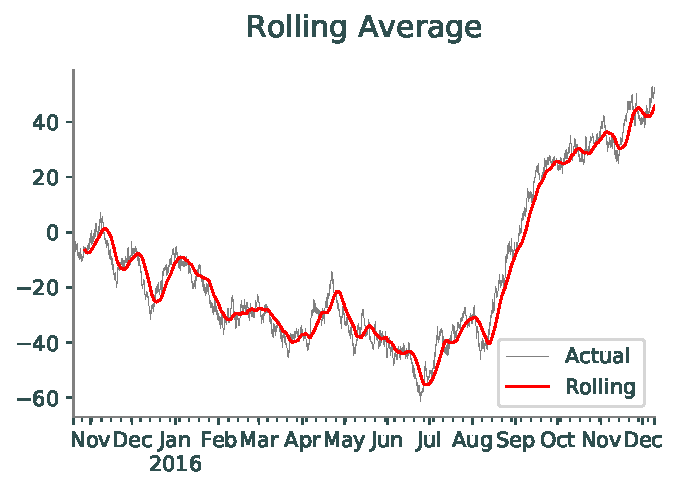
\includegraphics[width=\textwidth]{figures/moving_rolling.pdf}
    \caption{}
    \label{fig:pandas-ts-moving-rolling}
\end{subfigure}
%
\begin{subfigure}{.49\textwidth}
    \centering
    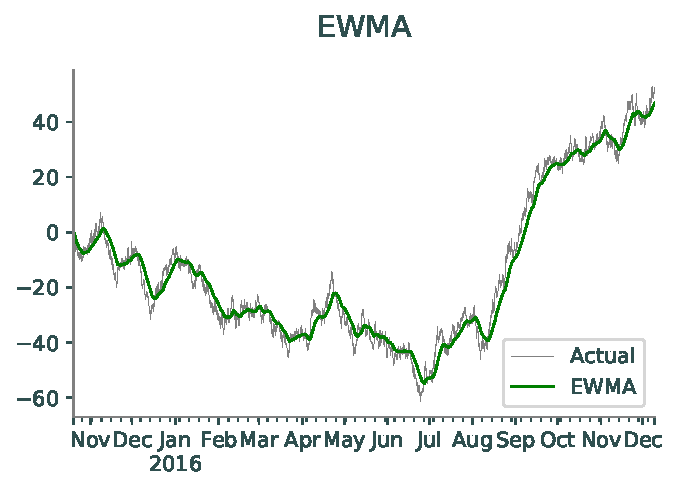
\includegraphics[width=\textwidth]{figures/moving_ewma.pdf}
    \caption{}
    \label{fig:pandas-ts-moving-ewma}
\end{subfigure}
\caption{Rolling average and EWMA.}
\end{figure}

\begin{lstlisting}
ax2 = plt.subplot(121)
s.plot(color="gray", lw=.3, ax=ax2)
s.ewm(span=200).mean().plot(color='g', lw=1, ax=ax2)
ax2.legend(["Actual", "EWMA"], loc="lower right")
ax2.set_title("EWMA")
\end{lstlisting}

\begin{problem}
Plot the following from the DJIA dataset with a window or span of 30, 120, and 365.
\begin{itemize}
    \item The original data points.
    \item Rolling average.
    \item Exponential average.
    \item Minimum rolling values.
    \item Maximum rolling values.
\end{itemize}
Describe how varying the length of the window changes the approximation to the data.
\end{problem}
